\documentclass[11pt,a4paper]{article}
\usepackage[margin=2.2cm]{geometry}
\usepackage{graphicx}
\usepackage{booktabs}
\usepackage{longtable}
\usepackage{amssymb}
\usepackage{hyperref}
\usepackage{caption}
\usepackage{enumitem}
\usepackage{xcolor}
\graphicspath{{figures/}}
\hypersetup{colorlinks=true,linkcolor=blue!50!black,urlcolor=blue!50!black}
\title{GPT-6 Astra on Complex Engineering Drawing Prompts:\\Text-to-SVG Evaluation and Failure Analysis}
\author{SVG Patch Lab --- generation eval \texttt{engineering\_v1}}
\date{11 September 2026}

\begin{document}
\maketitle

\begin{abstract}
We evaluated OpenAI's \texttt{gpt-6-astra} on 20 engineering drawing prompts spanning mechanical detail drawings, electrical and digital schematics, process and fluid-power diagrams, structural analysis diagrams, and architectural sections. Each prompt asked for a complete, self-contained SVG. All 20 outputs parsed as valid SVG, passed every structural must-have check (93/93), and survived visual review with \textbf{zero hard failures}. Four drawings show minor drafting-convention deviations. The run cost \$2.30 at \texttt{reasoning\_effort=low}, averaging 2251 output tokens and 44\,s per drawing. The most consequential failure modes we observed were not in Astra's drawings but in the evaluation setup: reasoning models can spend the whole output budget on hidden reasoning and return nothing, and naive structural checks produce false positives.
\end{abstract}

\section{Setup}
\begingroup\sloppy
\begin{description}[style=nextline,leftmargin=2em]
  \item[Model] \texttt{gpt-6-astra} via \url{https://api.openai.com/v1/chat/completions} (direct). The Experiential gateway route was also wired, but the model's platform-funded lane was purchase-gated at test time.
  \item[Request] Body fields: \texttt{model}, \texttt{messages}, \texttt{max\_completion\_tokens=16000}, \texttt{reasoning\_effort="low"}. No \texttt{temperature} or \texttt{top\_p} (the model rejects them). Single user message; no system prompt, no tools, no streaming.
  \item[Prompt template] \texttt{svgpatchlab/prompt\_templates/generation\_v1.txt}: return only an SVG document; declare \texttt{xmlns} and \texttt{viewBox}; built-in elements only; explicit colours; label parts and dimensions with \texttt{<text>}.
  \item[Harness] \texttt{scripts/eval\_generation.py} $\rightarrow$ \texttt{svgpatchlab/eval/generation.py}. Extracts the first \texttt{<svg>\ldots</svg>} (fenced or bare), parses with the project's hardened XML parser, runs declarative checks, classifies failures, and writes \texttt{results.jsonl}, \texttt{summary.json}, \texttt{outputs/*.svg}, and an HTML contact sheet with failures first.
  \item[Failure taxonomy] \texttt{truncated} (finish\_reason = length), \texttt{no\_svg}, \texttt{parse\_error}, \texttt{render\_error}, \texttt{blank\_render}, and \texttt{checks\_failed}; then manual visual review.
  \item[Rendering] PNG figures in this report were produced with macOS QuickLook (\texttt{qlmanage}). CairoSVG was unavailable (no native cairo), so automatic blank-render detection was off for this run.
  \item[Pricing] \$10/M input, \$50/M output tokens (OpenAI list; identical on the gateway's platform lane). Reasoning tokens are billed as output.
\end{description}
\endgroup

\section{Results}
\subsection{Aggregate}
\begin{center}
\begin{tabular}{lr}
\toprule
Prompts & 20 \\
Valid SVG / structural checks passed & 20/20 \quad (93/93 checks) \\
Hard failures after visual review & 0 \\
Minor convention deviations & 4 \\
Input tokens (total) & 4686 \\
Output tokens (total, incl.\ reasoning) & 45024 \\
\quad of which reasoning & 7311 \\
Mean output tokens / drawing & 2251 \\
Mean latency / drawing & 43.8\,s \\
Total cost & \$2.30 \quad (\$0.115 / drawing) \\
\bottomrule
\end{tabular}
\end{center}

\subsection{Per-prompt}
$^{*}$ = passes with a minor deviation, discussed in Section~\ref{sec:failures}.
\begin{longtable}{llrrrll}
\toprule
Prompt & Domain & Out tok & Reason. & s & Checks & Verdict \\
\midrule
\endhead
\texttt{flange\_bolt\_circle} & Mech. & 1559 & 342 & 33 & 5/5 & Pass \\
\texttt{rc\_lowpass\_schematic} & Elec. & 821 & 0 & 15 & 5/5 & Pass \\
\texttt{spur\_gear\_12t} & Mech. & 2319 & 710 & 54 & 5/5 & Pass$^{*}$ \\
\texttt{warren\_truss} & Struct. & 2150 & 200 & 40 & 4/4 & Pass \\
\texttt{bracket\_three\_view} & Mech. & 2304 & 388 & 45 & 5/5 & Pass \\
\texttt{pid\_pump\_loop} & Process & 2681 & 0 & 44 & 5/5 & Pass$^{*}$ \\
\texttt{beam\_shear\_moment} & Struct. & 2832 & 308 & 55 & 4/4 & Pass \\
\texttt{half\_adder\_logic} & Digital & 962 & 334 & 27 & 5/5 & Pass \\
\texttt{ibeam\_section} & Struct. & 1958 & 449 & 38 & 5/5 & Pass \\
\texttt{hydraulic\_circuit} & Fluid & 2757 & 509 & 55 & 4/4 & Pass \\
\texttt{floor\_plan\_studio} & Arch. & 2647 & 502 & 50 & 5/5 & Pass \\
\texttt{hex\_bolt\_side} & Mech. & 1769 & 268 & 33 & 4/4 & Pass$^{*}$ \\
\texttt{pcb\_footprint\_soic8} & PCB & 1999 & 362 & 40 & 4/4 & Pass \\
\texttt{planetary\_gearset} & Mech. & 3476 & 683 & 69 & 4/4 & Pass \\
\texttt{pipe\_isometric} & Piping & 2130 & 349 & 43 & 4/4 & Pass \\
\texttt{shell\_tube\_hx} & Process & 2192 & 241 & 43 & 5/5 & Pass \\
\texttt{staircase\_section} & Arch. & 2594 & 512 & 50 & 5/5 & Pass \\
\texttt{compression\_spring} & Mech. & 2389 & 512 & 47 & 4/4 & Pass$^{*}$ \\
\texttt{three\_phase\_motor\_starter} & Elec. & 2910 & 366 & 50 & 5/5 & Pass \\
\texttt{dimensioned\_plate} & Mech. & 2575 & 276 & 44 & 6/6 & Pass \\
\bottomrule
\end{longtable}

\begin{figure}[p]
  \centering
  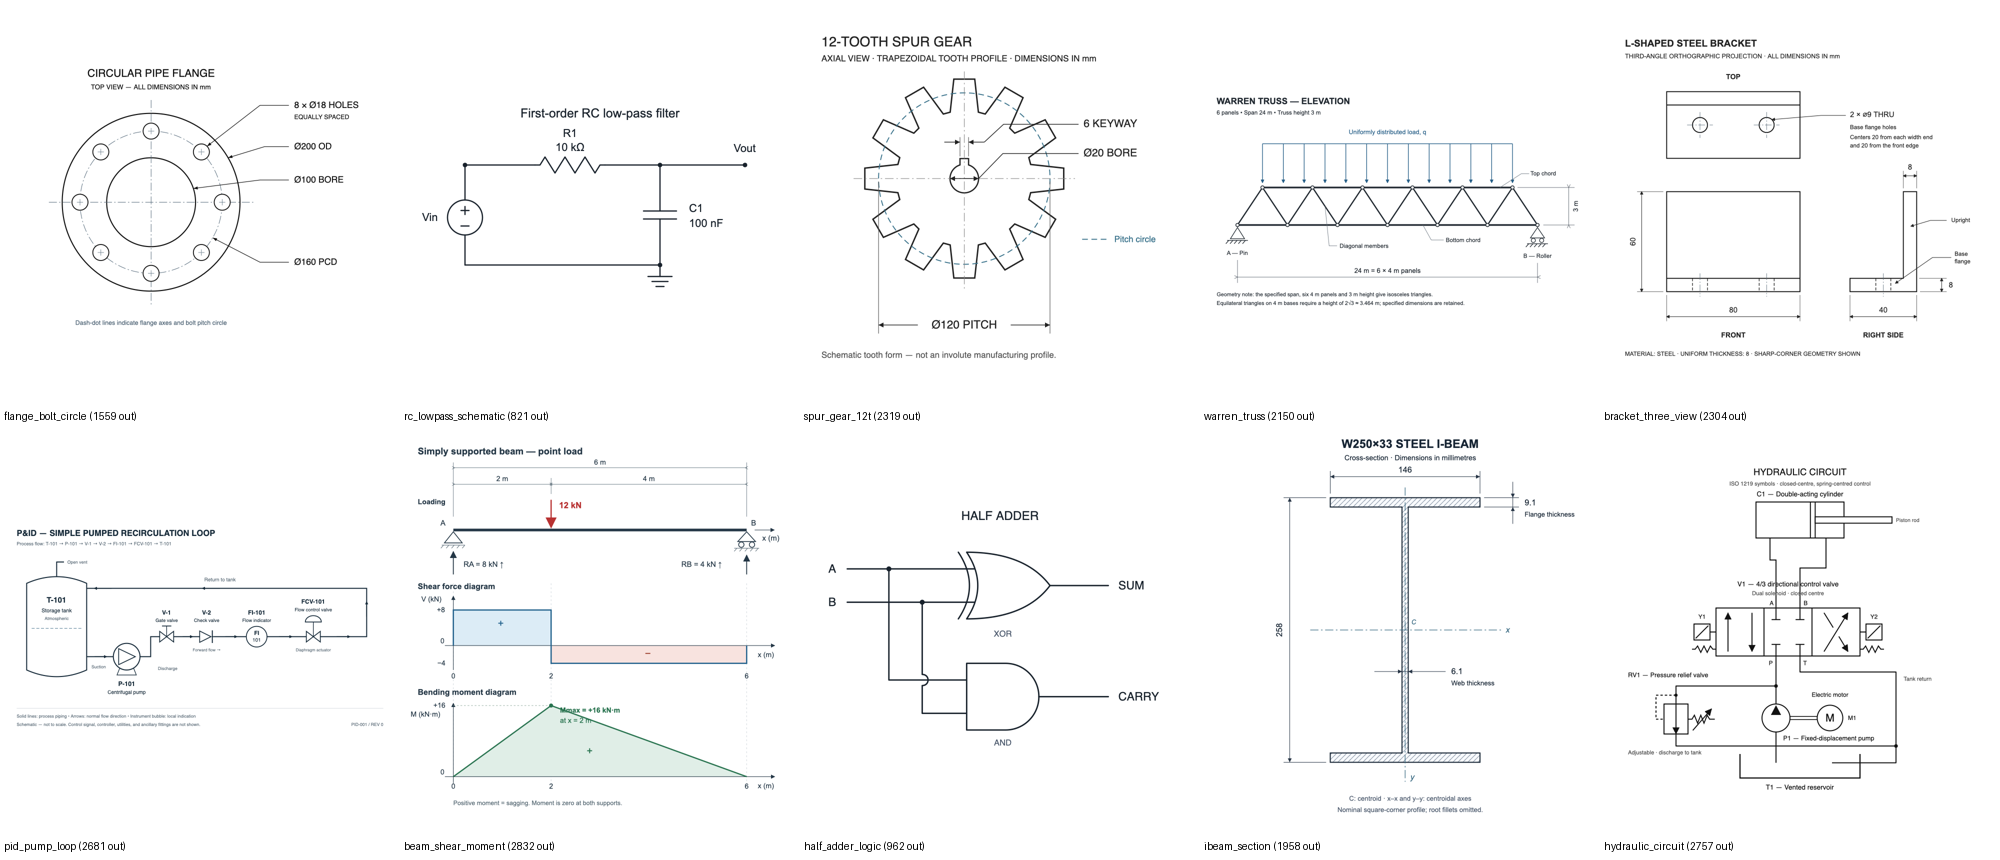
\includegraphics[width=\textwidth]{contact-1.png}\\[6pt]
  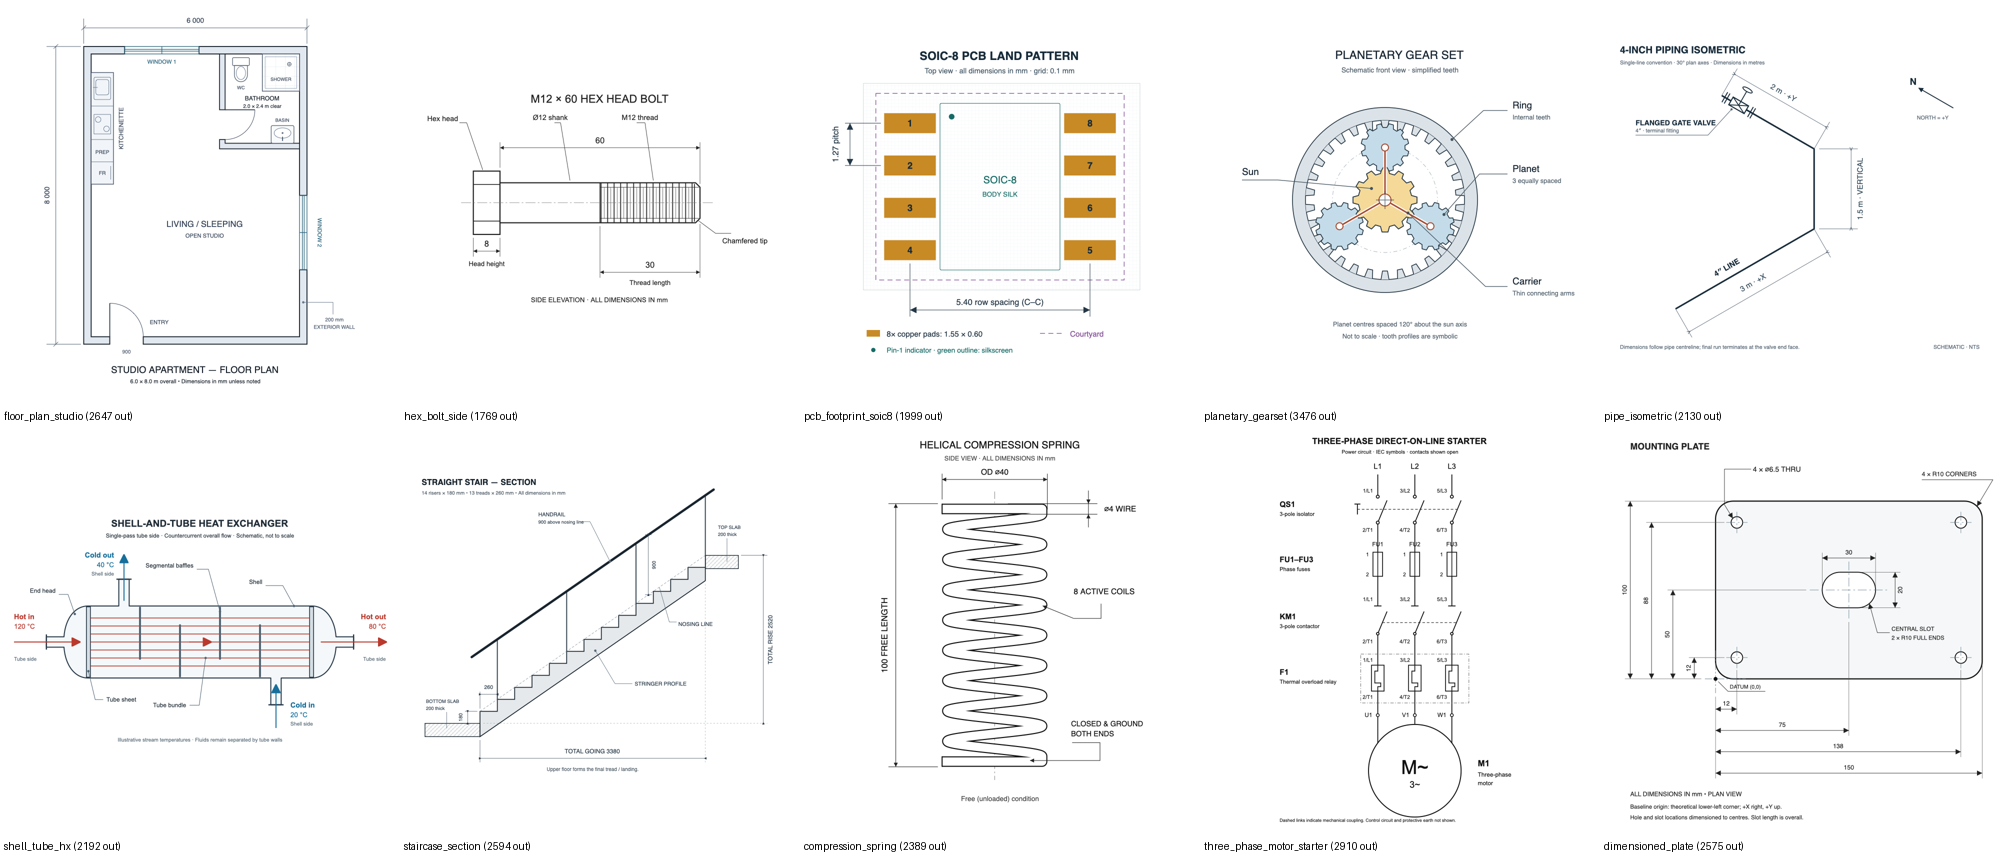
\includegraphics[width=\textwidth]{contact-2.png}
  \caption{All 20 drawings in prompt order (left to right, top to bottom), rendered from the SVG output without post-processing.}
  \label{fig:contact}
\end{figure}

\section{What Astra got right}
Properties verified by reading the SVG sources, not only the renders:
\begin{itemize}
  \item \textbf{Numerical correctness.} Beam reactions $R_A=8$\,kN, $R_B=4$\,kN and $M_{\max}=16$\,kN$\cdot$m for a 12\,kN load at 2\,m on a 6\,m span are exactly right, and the shear and moment diagrams are drawn to those values (Fig.~\ref{fig:beam}). Stair arithmetic is right (14 risers $\times$ 180 = 2520; 13 treads $\times$ 260 = 3380) and the profile path contains exactly 14 vertical and 13 horizontal segments. The plate's baseline dimensions (12/75/138/150 and 12/50/88/100) are consistent with the requested hole and slot positions.
  \item \textbf{Counted geometry.} The spur gear outline has 48 vertices, i.e.\ 12 trapezoidal teeth. The flange has 8 holes on the pitch circle; the SOIC-8 footprint has 8 pads numbered in the correct counter-clockwise order.
  \item \textbf{Drafting conventions.} Dash-dot centrelines; dashed hidden lines in the correct view; third-angle view placement; the ASME schematic thread convention (alternating thick full-height and thin short lines, implemented as an SVG \texttt{<pattern>}); section hatching clipped to the I-beam shape; filled arrowheads via \texttt{<marker>}; ISO~1219 4/3 closed-centre valve envelope with blocked centre ports; IEC terminal numbering (1L1/2T1\ldots) on the DOL starter.
  \item \textbf{Prompt sanity checking.} For the Warren truss the prompt's numbers are mutually inconsistent (six 4\,m equilateral panels imply a 3.46\,m height, not 3\,m). Astra drew the specified dimensions and added a note explaining the discrepancy rather than silently picking one.
  \item \textbf{Output discipline.} Every reply was a bare SVG document with no prose or fences; every root carried \texttt{xmlns} and \texttt{viewBox}; no external references.
\end{itemize}

\begin{figure}[t]
  \centering
  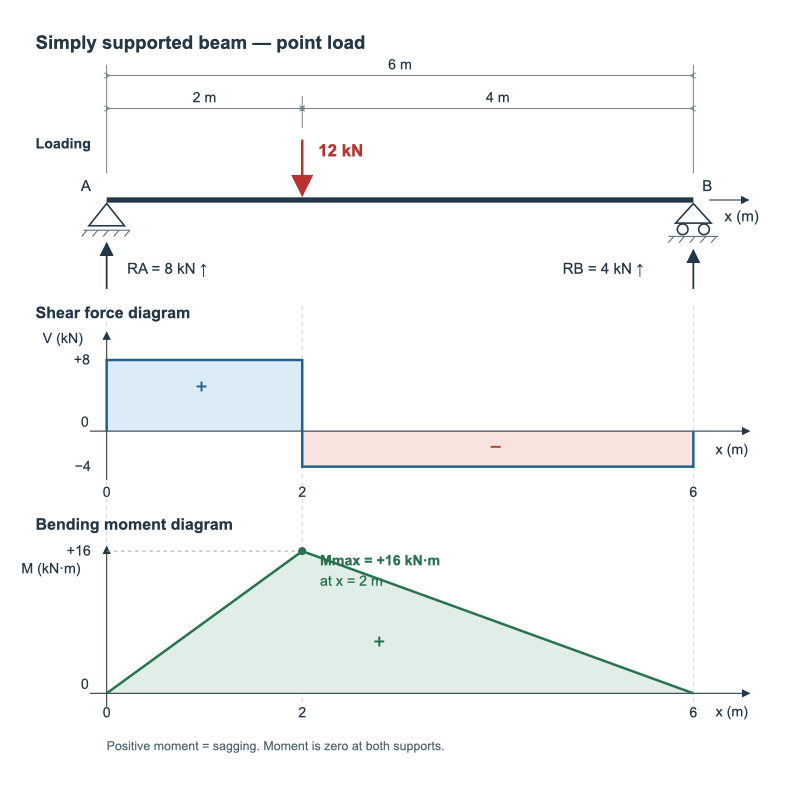
\includegraphics[width=0.48\textwidth]{beam_shear_moment.png}\hfill
  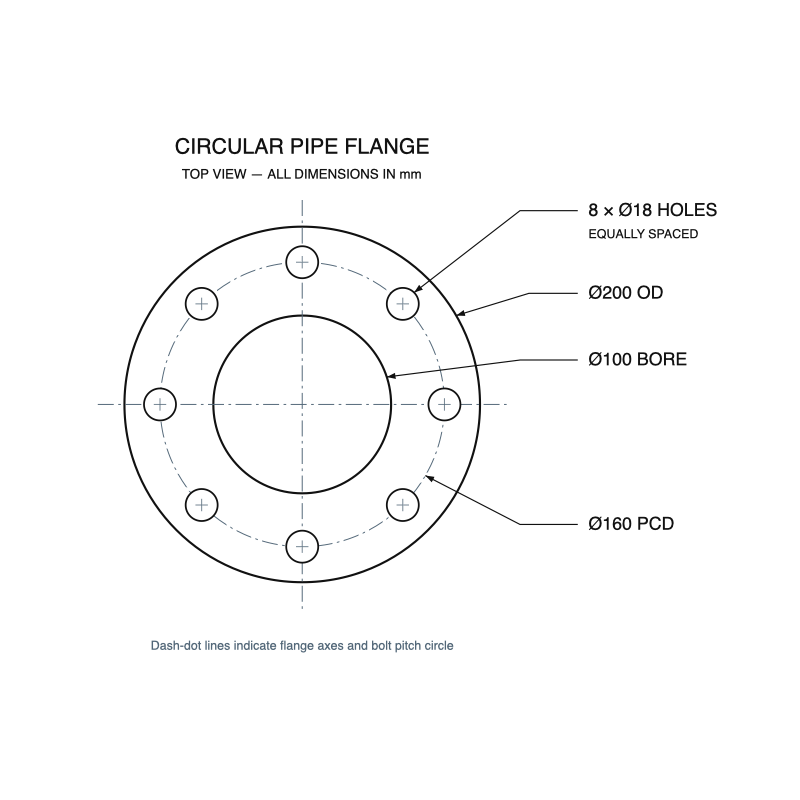
\includegraphics[width=0.48\textwidth]{flange_bolt_circle.png}
  \caption{Left: shear and bending-moment diagrams with correct reactions and maximum moment. Right: flange with pitch circle, centrelines and leader dimensions.}
  \label{fig:beam}
\end{figure}

\section{Failure analysis}\label{sec:failures}
\subsection{Astra: minor drafting deviations (4 of 20)}
None of these fail a structural check; all were found only by visual review.
\begin{enumerate}
\item \texttt{pid\_pump\_loop}: Pump drawn with the fluid-power circle-and-triangle glyph, not the ISA centrifugal-pump symbol.
\item \texttt{compression\_spring}: Coils are a rounded zigzag ribbon, not a helix projection; the prompt asked for ``not just a zigzag''.
\item \texttt{spur\_gear\_12t}: Keyway width has dimension arrows but no numeral at them; the value appears only in the leader label.
\item \texttt{hex\_bolt\_side}: Shank $\varnothing$12 given as a leader note rather than a dimension line.
\end{enumerate}
The two with substance are the P\&ID pump glyph (a symbol-vocabulary confusion between fluid-power and process-instrumentation standards) and the spring, where the model satisfied the letter of ``sinuous outline'' with a rounded zigzag rather than the overlapping elliptical arcs of a true helix side view (Fig.~\ref{fig:minor}). The other two are dimensioning omissions a checker would mark up, not errors of understanding.

\begin{figure}[t]
  \centering
  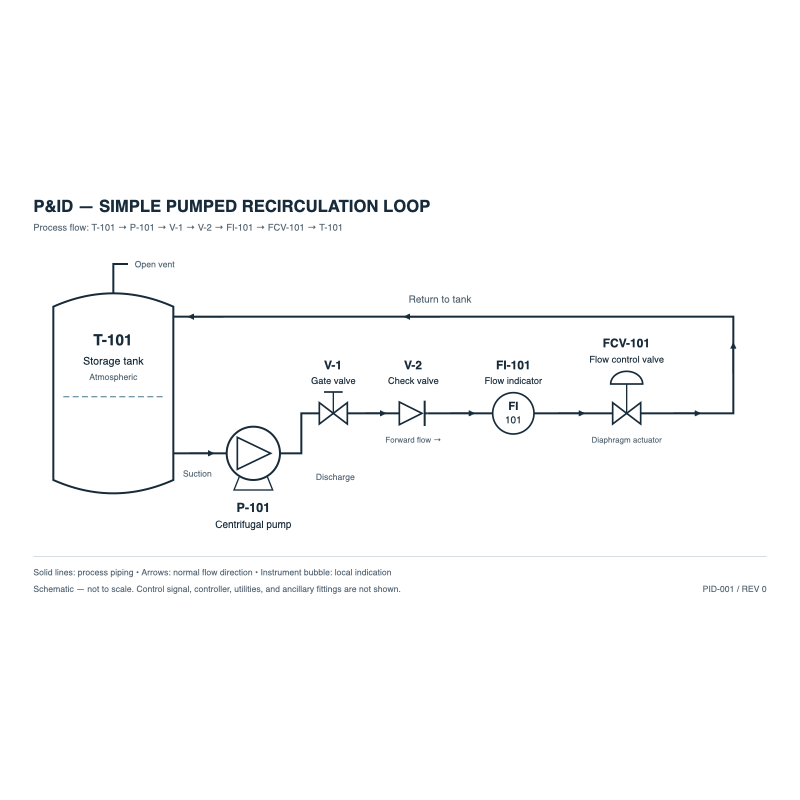
\includegraphics[width=0.56\textwidth]{pid_pump_loop.png}\hfill
  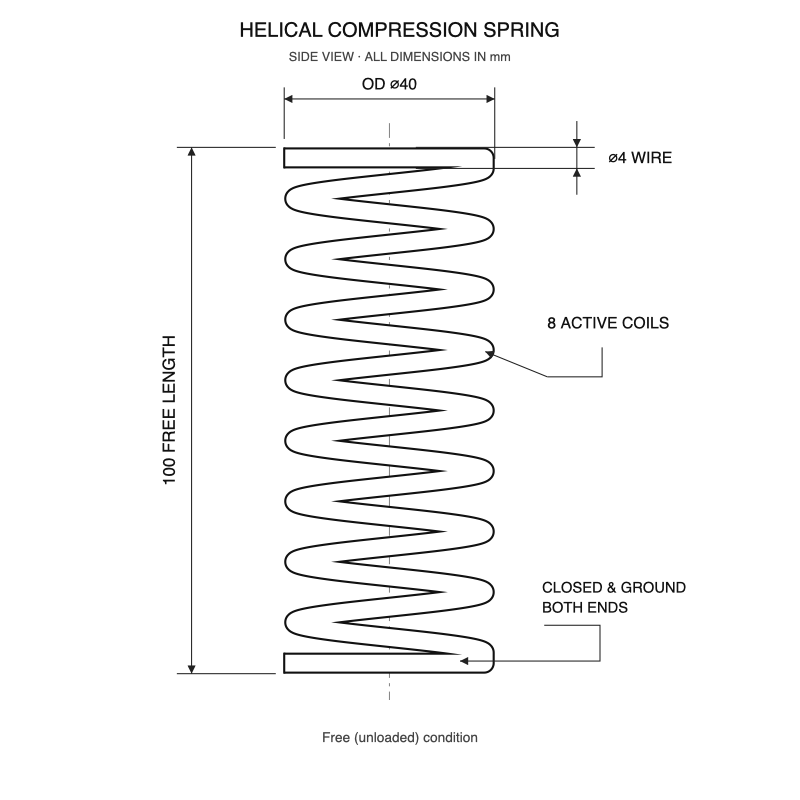
\includegraphics[width=0.36\textwidth]{compression_spring.png}
  \caption{Left: P\&ID with the pump drawn as a fluid-power symbol (circle and triangle) rather than an ISA centrifugal pump. Right: compression spring drawn as a rounded zigzag ribbon.}
  \label{fig:minor}
\end{figure}

\subsection{Evaluation-side failure modes (the ones that actually bit)}
\begin{enumerate}
  \item \textbf{Reasoning-budget exhaustion.} In the harness dry run on a different reasoning model (\texttt{qwen3.8-27b} via the gateway, cap 8192) one prompt returned \texttt{finish\_reason=length} with \emph{zero} visible characters: the entire budget went to hidden reasoning. For Astra we therefore set \texttt{max\_completion\_tokens=16000} and \texttt{reasoning\_effort=low}; Astra then used 0--710 reasoning tokens per drawing and never approached the cap. Any evaluation of a reasoning model must record \texttt{finish\_reason} and \texttt{completion\_tokens\_details.reasoning\_tokens}, or truncation is indistinguishable from refusal.
  \item \textbf{Structural-check false positive.} The 3-prompt smoke run flagged \texttt{spur\_gear\_12t} as \texttt{checks\_failed} because the check demanded two \texttt{<circle>} elements and Astra drew the pitch circle and bore as \texttt{<path>} arcs. The drawing was correct; the check was loosened to accept \texttt{circle}/\texttt{path}/\texttt{ellipse}. Element-type checks measure encoding choices, not drawing correctness: they are floors for ``did it draw anything'', not quality metrics.
  \item \textbf{No automatic blank detection.} Without a rasteriser in the loop, a syntactically valid SVG that renders empty (all geometry outside the \texttt{viewBox}, or neither filled nor stroked) would pass. None occurred here, but the run cannot prove that automatically.
  \item \textbf{Single sample.} Each prompt was generated once. Zero failures at $n=1$ bounds the per-prompt failure rate only loosely; a three-sample run would separate ``can'' from ``usually does''.
\end{enumerate}

\subsection{Cost and latency profile}
Output tokens ranged from 821 (RC filter) to 3476 (planetary gear set); reasoning tokens from 0 to 710. Per-drawing cost ranged \$0.04--\$0.18. Latency ranged 15--69\,s and tracks output length almost linearly (roughly 50 tokens/s), so wall-clock is dominated by SVG verbosity rather than thinking. At \texttt{reasoning\_effort=low} the full 20-prompt pass cost \$2.30, under the \$8--12 pre-run estimate.

\section{Limitations and next steps}
\begin{itemize}
  \item The prompt set is authored by the evaluator, not drawn from real engineering work orders; the checks are hand-written floors.
  \item Run with \texttt{--samples 3} to measure consistency; try \texttt{reasoning\_effort=medium} on the four starred prompts to see whether the deviations are effort-limited.
  \item Add harder prompts: multi-view assemblies with section views, GD\&T frames, ladder logic with cross-references, drawings requiring computed geometry (involute tooth profiles, true isometric ellipses).
  \item Add a vision-model judge scoring each render 1--5 against its prompt, and a CairoSVG rasteriser (\texttt{brew install cairo}) for blank-render detection.
\end{itemize}

\appendix
\section{Prompts}
\begin{description}[style=nextline,leftmargin=1em]
\item[\texttt{flange\_bolt\_circle}] Top view of a circular pipe flange: outer diameter 200 mm, bore 100 mm, 8 bolt holes of 18 mm on a 160 mm pitch circle. Show the pitch circle as a dashed centerline, a horizontal and vertical centerline, and dimension the OD, bore, PCD and one hole with leader lines and arrowheads.
\item[\texttt{rc\_lowpass\_schematic}] Electrical schematic of a first-order RC low-pass filter: voltage source Vin on the left, series resistor R1 = 10 k$\Omega$, shunt capacitor C1 = 100 nF to ground, output node labelled Vout on the right. Use standard schematic symbols (zigzag resistor, parallel-plate capacitor, ground symbol), junction dots, and component labels.
\item[\texttt{spur\_gear\_12t}] A 12-tooth spur gear viewed along its axis, pitch diameter 120 mm, with a 20 mm bore and a 6 mm keyway. Draw the tooth profile as a closed outline (trapezoidal teeth are acceptable), show the pitch circle as a dashed line, and dimension the pitch diameter and bore.
\item[\texttt{warren\_truss}] Elevation of a Warren truss bridge span with 6 panels, span 24 m, height 3 m. Draw top and bottom chords, diagonal members forming equilateral triangles, pin support at the left and roller support at the right (standard symbols), a uniformly distributed load shown as an arrow row on the top chord, and dimension the span and height.
\item[\texttt{bracket\_three\_view}] Third-angle orthographic projection (front, top, right side views) of an L-shaped steel bracket: 80 mm wide, 60 mm tall, 40 mm deep, 8 mm thick, with two 9 mm through-holes in the base flange. Align the views correctly, use hidden lines (dashed) for the holes where appropriate, and dimension the overall sizes.
\item[\texttt{pid\_pump\_loop}] P\&ID of a simple pumped loop: storage tank T-101 feeding centrifugal pump P-101, discharge through gate valve V-1, check valve V-2, flow indicator FI-101, and a control valve FCV-101 back to the tank. Use ISA-style symbols (tank outline, pump circle with triangle, valve bowties, instrument bubbles with tag text) and label every item.
\item[\texttt{beam\_shear\_moment}] A simply supported beam of length 6 m with a 12 kN point load at 2 m from the left support. Draw three vertically stacked, aligned diagrams: the loaded beam with reactions labelled RA and RB, the shear force diagram, and the bending moment diagram, each with axis labels and the key values (reactions, maximum moment) annotated.
\item[\texttt{half\_adder\_logic}] Logic diagram of a half adder: inputs A and B, an XOR gate producing SUM and an AND gate producing CARRY. Use distinct IEEE/ANSI gate shapes (curved-back XOR with the extra input arc, D-shaped AND), wire fan-out with junction dots, and label inputs and outputs.
\item[\texttt{ibeam\_section}] Cross-section of a W250x33 steel I-beam: depth 258 mm, flange width 146 mm, flange thickness 9.1 mm, web thickness 6.1 mm. Draw the section with section-line hatching (45$^{\circ}$ lines clipped to the shape), the centroidal axes as dash-dot lines, and dimension depth, flange width, and both thicknesses.
\item[\texttt{hydraulic\_circuit}] ISO 1219 hydraulic circuit: reservoir, fixed-displacement pump driven by an electric motor, pressure relief valve back to tank, a 4/3 directional control valve (closed-centre, solenoid operated), and a double-acting cylinder. Draw the valve envelope as three adjacent boxes with flow-path arrows, use proper reservoir and cylinder symbols, and label each component.
\item[\texttt{floor\_plan\_studio}] Architectural floor plan of a 6 m x 8 m studio apartment: exterior walls 200 mm thick drawn as double lines, an entry door with swing arc, two windows, a bathroom 2 m x 2.4 m in one corner with toilet, basin and shower, a kitchenette counter along one wall, and overall dimension strings on two sides.
\item[\texttt{hex\_bolt\_side}] Side elevation of an M12 x 60 hex head bolt: hex head 8 mm tall with the middle facet visible as a rectangle and the two outer facets as narrower rectangles, a 12 mm shank, 30 mm of thread shown as the conventional thread representation (alternating full and thin lines), and a chamfered tip. Dimension the length, thread length, and head height.
\item[\texttt{pcb\_footprint\_soic8}] PCB land pattern for an SOIC-8 package: 8 rectangular copper pads 1.55 mm x 0.6 mm at 1.27 mm pitch in two rows 5.4 mm apart, a silkscreen outline of the body, a pin-1 indicator dot, courtyard boundary as a dashed rectangle, and pad numbers. Use a 0.1 mm grid scale and dimension the pitch and row spacing.
\item[\texttt{planetary\_gearset}] Schematic front view of a planetary gear set: a sun gear in the centre, three equally spaced planet gears, a ring gear as an internal-toothed annulus, and a planet carrier drawn as thin arms connecting planet centres. Teeth may be simplified to notches. Label sun, planet, ring and carrier.
\item[\texttt{pipe\_isometric}] Isometric piping sketch: a 4-inch line runs 3 m in the +X direction, rises 1.5 m vertically, then runs 2 m in the +Y direction, ending at a flanged gate valve. Use single-line isometric convention with 30$^{\circ}$ axes, show the flanges as short perpendicular double ticks, put a north arrow, and dimension each run.
\item[\texttt{shell\_tube\_hx}] Process schematic of a shell-and-tube heat exchanger: horizontal shell with two tube-side nozzles on the end heads and two shell-side nozzles on top and bottom of the shell, a tube bundle drawn as several parallel lines, baffles as vertical segments, and flow arrows with stream labels (hot in, hot out, cold in, cold out) and temperatures.
\item[\texttt{staircase\_section}] Section through a straight residential staircase with 14 risers of 180 mm and treads of 260 mm, a handrail at 900 mm above the nosing line, and floor slabs 200 mm thick at top and bottom. Draw the stringer profile, hatch the slabs, and dimension total rise, total going, one riser and one tread.
\item[\texttt{compression\_spring}] Side view of a helical compression spring with 8 active coils, wire diameter 4 mm, outer diameter 40 mm, free length 100 mm, with closed and ground ends. Draw the coils as a continuous sinuous outline (not just a zigzag), and dimension free length, OD and wire diameter.
\item[\texttt{three\_phase\_motor\_starter}] Power circuit for a three-phase direct-on-line motor starter: L1, L2, L3 supply, a three-pole isolator, three fuses, a three-pole contactor KM1, a thermal overload relay F1, and motor M1 drawn as a circle with the M$\sim$ symbol. Use IEC symbols, draw the three phases as parallel vertical lines, and label all components and terminals.
\item[\texttt{dimensioned\_plate}] A rectangular mounting plate 150 mm x 100 mm with 10 mm corner radii, four 6.5 mm holes 12 mm in from each edge, and a central 30 mm x 20 mm rectangular slot with full-radius ends. Fully dimension it to a datum at the lower-left corner using baseline dimensioning with extension lines, dimension lines and filled arrowheads.
\end{description}

\section{Reproduction}
\begin{verbatim}
set -a; . ./.env; set +a   # provides OPENAI_API_KEY
python3 scripts/eval_generation.py \
  --model-config configs/models/openai-gpt-6-astra.json \
  --no-render --price-in 10 --price-out 50 \
  --output-dir runs/gen-astra-v1
open runs/gen-astra-v1/index.html
\end{verbatim}
\end{document}
